\documentclass{article}
\usepackage[landscape, twocolumn, columnsep=1.5cm,margin=0.75in]{geometry}
\usepackage{amsmath}
\usepackage{graphicx}
\usepackage{wrapfig}
\usepackage[colorlinks=true, allcolors=blue]{hyperref}
\usepackage[english]{babel}
\usepackage{float}
\usepackage{blindtext}
\usepackage{mathtools}
\DeclarePairedDelimiter\bra{\langle}{\rvert}
\DeclarePairedDelimiter\ket{\lvert}{\rangle}
\usepackage[colorlinks=true, allcolors=blue]{hyperref}
\usepackage{xcolor}
\renewcommand{\thesubsection}{\thesection.\alph{subsection}}
\usepackage{gensymb}
\usepackage{tabularx}
\usepackage{algorithm}
\usepackage{algpseudocode}
\usepackage{subcaption}


\title{Computational HW 1}

\author{Michael Bibbs}
\begin{document}
	\maketitle
	\section*{Radioactive Decay}
	\section{Introduction}
	Consider a radioactive decay problem involving two types of nuclei, $A$ and $B$, with populations $N_A(t)$ and $N_B(t)$. Suppose that type $A$ nuclei decay to form type $B$ nuclei, which then also decay, according to the differential equations
	\begin{equation}
		\frac{dN_A}{dt}=-\frac{N_A}{\tau_A}
	\end{equation}
	\begin{equation}
		\frac{dN_B}{dt}=\frac{N_A}{\tau_A}-\frac{N_B}{\tau_B}
	\end{equation}
	\\\indent Here, we assume that type A nuclei are naturally occurring, and type B are not. This paper focuses on determing the age of an object by measuring the amount of type A and B nuclei within the object. We then discuss the accuracy of the age based on the ratio of measured nuclei $N_B / N_A$
	\section{Methods}
	\indent The original Euler method is used. The form
	\[f(t+\Delta t)=f(t)+\frac{df}{dt}(t)\Delta t\]
	\indent is adapted into our coupled differential equations. We obtain the iteration relations
	\begin{equation}
		N_A(t+\Delta t) = N_A(t) -\frac{N_A(t)}{\tau_A}\Delta t
	\end{equation}
	\begin{equation}
		N_B(t+\Delta t) = N_B(t)+\left(\frac{N_A(t)}{\tau_A}-\frac{N_B(t)}{\tau_B}\right)\Delta t
	\end{equation}\\
	\indent The following parameters were initialized as such:
	\begin{enumerate}
		\item Initial Type A nuclei $N_A(0) = 1$~~~{\textit{\footnotesize (Note: this represents 100\% of the starting nuclei being type A.)}}
		\item Initial Type B nuclei $N_B(0) = 0$
		\item Type A Decay Constant $\tau_A$
		\item Type B Decay Constant $\tau_B$ 
		\item Nuclei ratio $r=N_B/N_A$
		\item Scaled time $T = t/\tau_A$
	\end{enumerate}
	
	\begin{minipage}{0.7\linewidth}
		\rule{\linewidth}{0.5pt}
		\refstepcounter{algorithm} 
		\textbf{Algorithm 1} Euler's Method
		
		\vspace{-0.5em}
		\rule{\linewidth}{0.5pt}
		
		\begin{algorithmic}
			\Require $t>0$
			\State $N_A \gets [1]$ \Comment{Initial Value}
			\State $N_B \gets [0]$ \Comment{Initial Value}
			\While{$t<t_{MAX}$}
			\State append $N_A(t)  -\frac{N_A(t)}{\tau_A}\Delta t$ to $N_A$
			\State append $N_B(t) +\left(\frac{N_A(t)}{\tau_A}-\frac{N_B(t)}{\tau_B}\right) \Delta t$
			\State $t \gets t + \Delta t$
			\EndWhile
			\State $r \gets N_B/N_A$\Comment{Element-Wise Division}
			\State \Return $r$
		\end{algorithmic}
		
		\rule{\linewidth}{0.5pt}
		\vspace{0.25mm}
	\end{minipage}
	\\The analytic solutions for the coupled differential equations (1),(2) are:
	\begin{equation}
		N_A(t)=e^{-t/\tau_A}
	\end{equation}
	\begin{equation}
		N_B(t)=\dfrac{\tau_B}{\tau_A-\tau_B}\left(e^{-t/\tau_A}-e^{-t/\tau_B}\right)
	\end{equation}\vspace{-1mm}
	\\\indent The above algorithm was used, in conjunction with the analytic solution (see Appendix A.) to test the accuracy of the iteration method and explore uncertainty in age of the observed object. No use of generative AI was used in this assignment.
	\begin{figure}[H]
		\centering
		\begin{subfigure}{0.5\textwidth}
			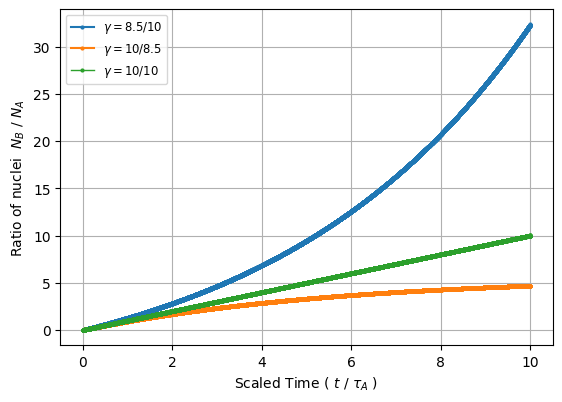
\includegraphics[width=0.9\linewidth]{fig6.png}
		\end{subfigure}
		\begin{subfigure}{0.5\textwidth}
			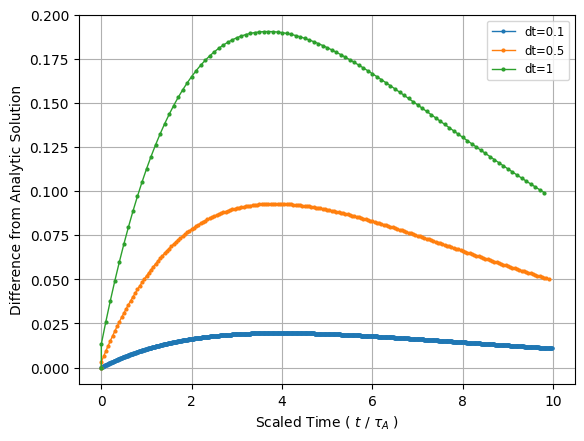
\includegraphics[width=0.9\linewidth]{fig7.png}
		\end{subfigure}
		\caption{Ratio of type B and type A nuclei over time, testing different\\ (a) decay constants $\gamma$, constant $\Delta t=0.01$~~\\(b) time steps $\Delta t$, constant $\gamma=10/8$ }
	\end{figure}
	\section{Results}
	Different decay ratios $\gamma = \tau_A/\tau/B$ were tested. Exponential bounded growth was observed with $\gamma>1$, unbounded growth with $\gamma<1$, and linear growth with $\gamma = 1$. 
	\\ \indent The ratios $r$ and analytic solutions are plotted against corresponding scaled times $T$, shown in Figure~1.a.\vspace{-1mm}
	\section{Discussion}
	The age of the object can be somewhat accurately determined based on the decay constant ratio $\gamma$. For ratio $\gamma<1$, accuracy decreases as scaled age $t/\tau_A$ increases. Due to the unbounded exponential growth, a variation in ratio $N_B/N_A$ corresponds with less variation in age. Early on, there is a large uncertainty, due to a slow initial growth. 
	\\ \indent On the other hand, with decay ratio $\gamma>1$, uncertainty increases with age. Initially, the nuclei ratio quickly plateaus, and slows down as the object ages. This corresponds with accurate dating early on, where only a small range of ages  lie within a region of ratios. Once the ratio flattens out, the ratio asymptotic value can be explained by a large range of ages. 
	\\ \indent with a decay constant ratio $\gamma=1$, there is little uncertainty in the age, as the decay ratio follows a perfectly linear line. This uncertainty is constant as the age increases due to this linear relationship. 
	\\\\ Euler's method showed consistent agreement with the analytical solution. Shown in Figure 1.b, the method used shows agreement with the exact solution for $\gamma>1$. Euler's method consistently over-estimated the numerical solution. 
	\\ \indent With low decay constants $\gamma<1$, this over-shooting grew as age increased, causing larger discrepancies between Euler's method and the analytic solution. 
	\section{Summary}
	Euler's Method proved to be very reliable in predicting the age of an object based on the ratio of $N_A$ and $N_B$ type nuclei within it. The time constant ratio $\gamma$ determined the decay behavior, which in turn provided varying results on age prediction accuracy. 
	\pagebreak
	\section*{Derivation of Analytical Solution}
	We start with the coupled differential equations:
	\[\frac{dN_A}{dt}=-\frac{N_A}{\tau_A}\]
	\[\frac{dN_B}{dt}=\frac{N_A}{\tau_A}-\frac{N_B}{\tau_B}\]
	The first can be easily seen:
	\[N_A'(t)=\frac{-1}{\tau_A}N_A(t)\rightarrow \boxed{N_A(t)=e^{-t/\tau_A}}\]
	For our case, the initial value is simply 1.
	\\ This result is then used for $N_B$:
	\[N_B'(t)=\frac{N_A(t)}{\tau_A}-\frac{N_B(t)}{\tau_B}\]
	\[N_B'(t)+\frac{N_B(t)}{\tau_B}=\frac{1}{\tau_A}e^{-t/\tau_A}\]
	We find the integrating factor:
	\[e^{\int{dt/\tau_B}}=e^{t/\tau_B}\]
	Multiply the ODE by this integrating factor:
	\[e^{t/\tau_B}N_B'(t)+\frac{1}{\tau_B}E^{t/\tau_B}N_B(t)=\frac{1}{\tau_A}e^{t/\tau_B-t/\tau_A}\]
	Recognize the chain rule:
	\[\frac{d}{dt}\left[e^{t/\tau_B}N_B(t)\right]=\frac{1}{\tau_A}e^{t/\tau_B-t/\tau_A}\]
	Integrate both sides:
	\[\int\frac{d}{dt}\left[e^{t/\tau_B}N_B(t)\right]dt=\int\frac{1}{\tau_A}e^{t/\tau_B-t/\tau_A}\]
	\[e^{t/\tau_B}B(t)=\dfrac{1/\tau_A}{1/\tau_B-1/\tau_A}\left[e^{t/\tau_B-t/\tau_A}-1\right]\]
	\[\boxed{B(t)=\dfrac{\tau_B}{\tau_A-\tau_B}\left(e^{-t/\tau_A}-e^{-t/\tau_B}\right)}\]
\end{document}
